\documentclass{standalone}
\usepackage{pgfplots}
\pgfplotsset{compat=1.18}
\usepgfplotslibrary{colorbrewer}
\pgfplotsset{cycle list/Set1-6}

\begin{document}

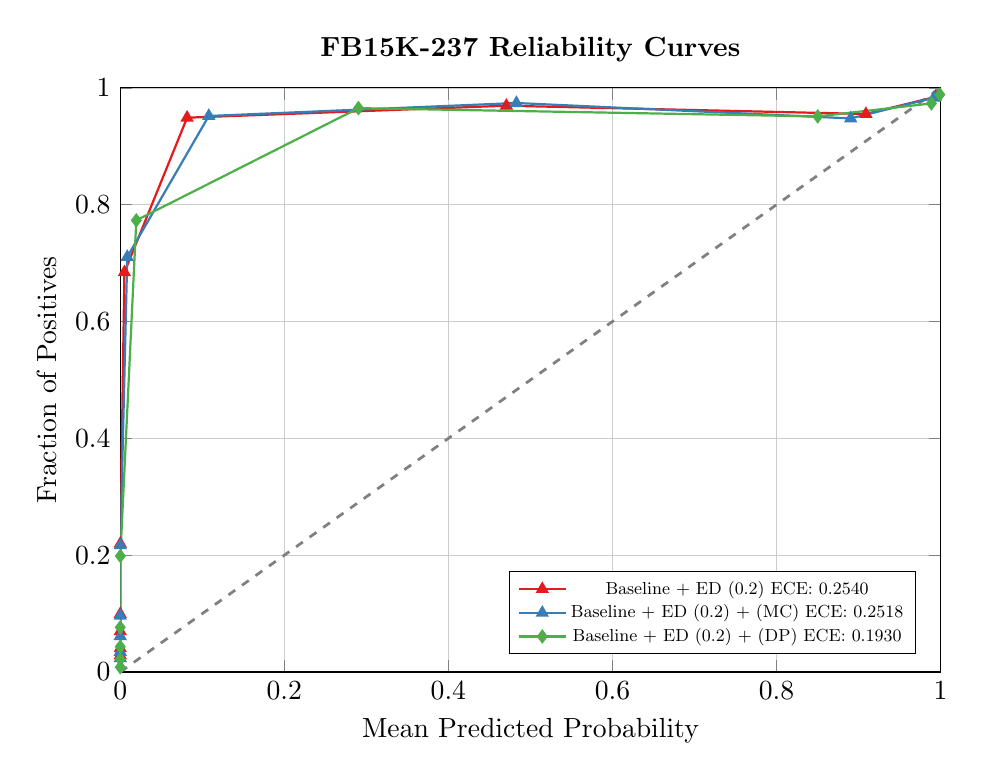
\begin{tikzpicture}
\begin{axis}[
    title={\textbf{FB15K-237 Reliability Curves}},
    xlabel={Mean Predicted Probability},
    ylabel={Fraction of Positives},
    xmin=0, xmax=1,
    ymin=0, ymax=1,
    xtick={0, 0.2, 0.4, 0.6, 0.8, 1.0},
    ytick={0, 0.2, 0.4, 0.6, 0.8, 1.0},
    legend pos= south east,
    legend style={nodes={scale=0.7, transform shape}, font=\small},
    grid=both,
    grid style={line width=.1pt, draw=gray!20},
    major grid style={line width=.2pt, draw=gray!40},
    width=12cm,
    height=9cm,
    cycle list name=Set1-6
]

% Perfectly Calibrated Line
\addplot [color=gray, dashed, line width=1pt, forget plot]
    coordinates {(0,0)(1,1)};

\addplot+[mark=triangle*, thick] coordinates {
    (4.21827188e-11, 0.02833415) (8.90112614e-09, 0.04055705) (2.61931652e-07, 0.06963108) (4.30301209e-06, 0.09919375)
    (8.06938248e-05, 0.21964329) (5.08208580e-03, 0.68433912) (8.14976601e-02, 0.94893721) (4.70707676e-01, 0.96946005)
    (9.08945809e-01, 0.95528952) (9.93830265e-01, 0.98461163)
};
\addlegendentry{Baseline + ED (0.2) ECE: 0.2540}

\addplot+[mark=triangle*, thick] coordinates {
    (1.44075803e-10, 0.02369321) (2.20232701e-08, 0.03444906) (5.51256726e-07, 0.06132421) (8.01007305e-06, 0.09626191)
    (1.38782212e-04, 0.21695578) (8.52853797e-03, 0.71048131) (1.07916471e-01, 0.95186904) (4.82877058e-01, 0.97410213)
    (8.90374851e-01, 0.94771561) (9.91898650e-01, 0.98314607)
};
\addlegendentry{Baseline + ED (0.2) + (MC) ECE: 0.2518}

\addplot+[mark=diamond*, thick] coordinates {
    (8.08637221e-11, 0.00830484) (1.27878564e-08, 0.02174444) (3.47365550e-07, 0.04324456) (5.52997593e-06, 0.07647203)
    (1.38037954e-04, 0.19863181) (1.95757910e-02, 0.77327144) (2.90354831e-01, 0.96530662) (8.50231506e-01, 0.95113609)
    (9.88813320e-01, 0.97336917) (9.99124482e-01, 0.98851979)
};
\addlegendentry{Baseline + ED (0.2) + (DP) ECE: 0.1930}


\end{axis}
\end{tikzpicture}

\end{document}